\usepackage{graphicx}
\usepackage{pgfpages}
\usepackage{hyperref}
\usetheme{metropolis}
\setbeamertemplate{background canvas}[vertical shading][top=white,bottom=cyan!30]
\setbeamertemplate{navigation symbols}{}

\setbeamertemplate{footline}{%
  \begin{beamercolorbox}[wd=\paperwidth,ht=2.5ex,dp=1ex,right]{footline}%
    Page \insertframenumber{} / \inserttotalframenumber
  \end{beamercolorbox}%
}

% Consistent Image (using ucam.png as originally provided)
\newcommand{\frametitleimage}{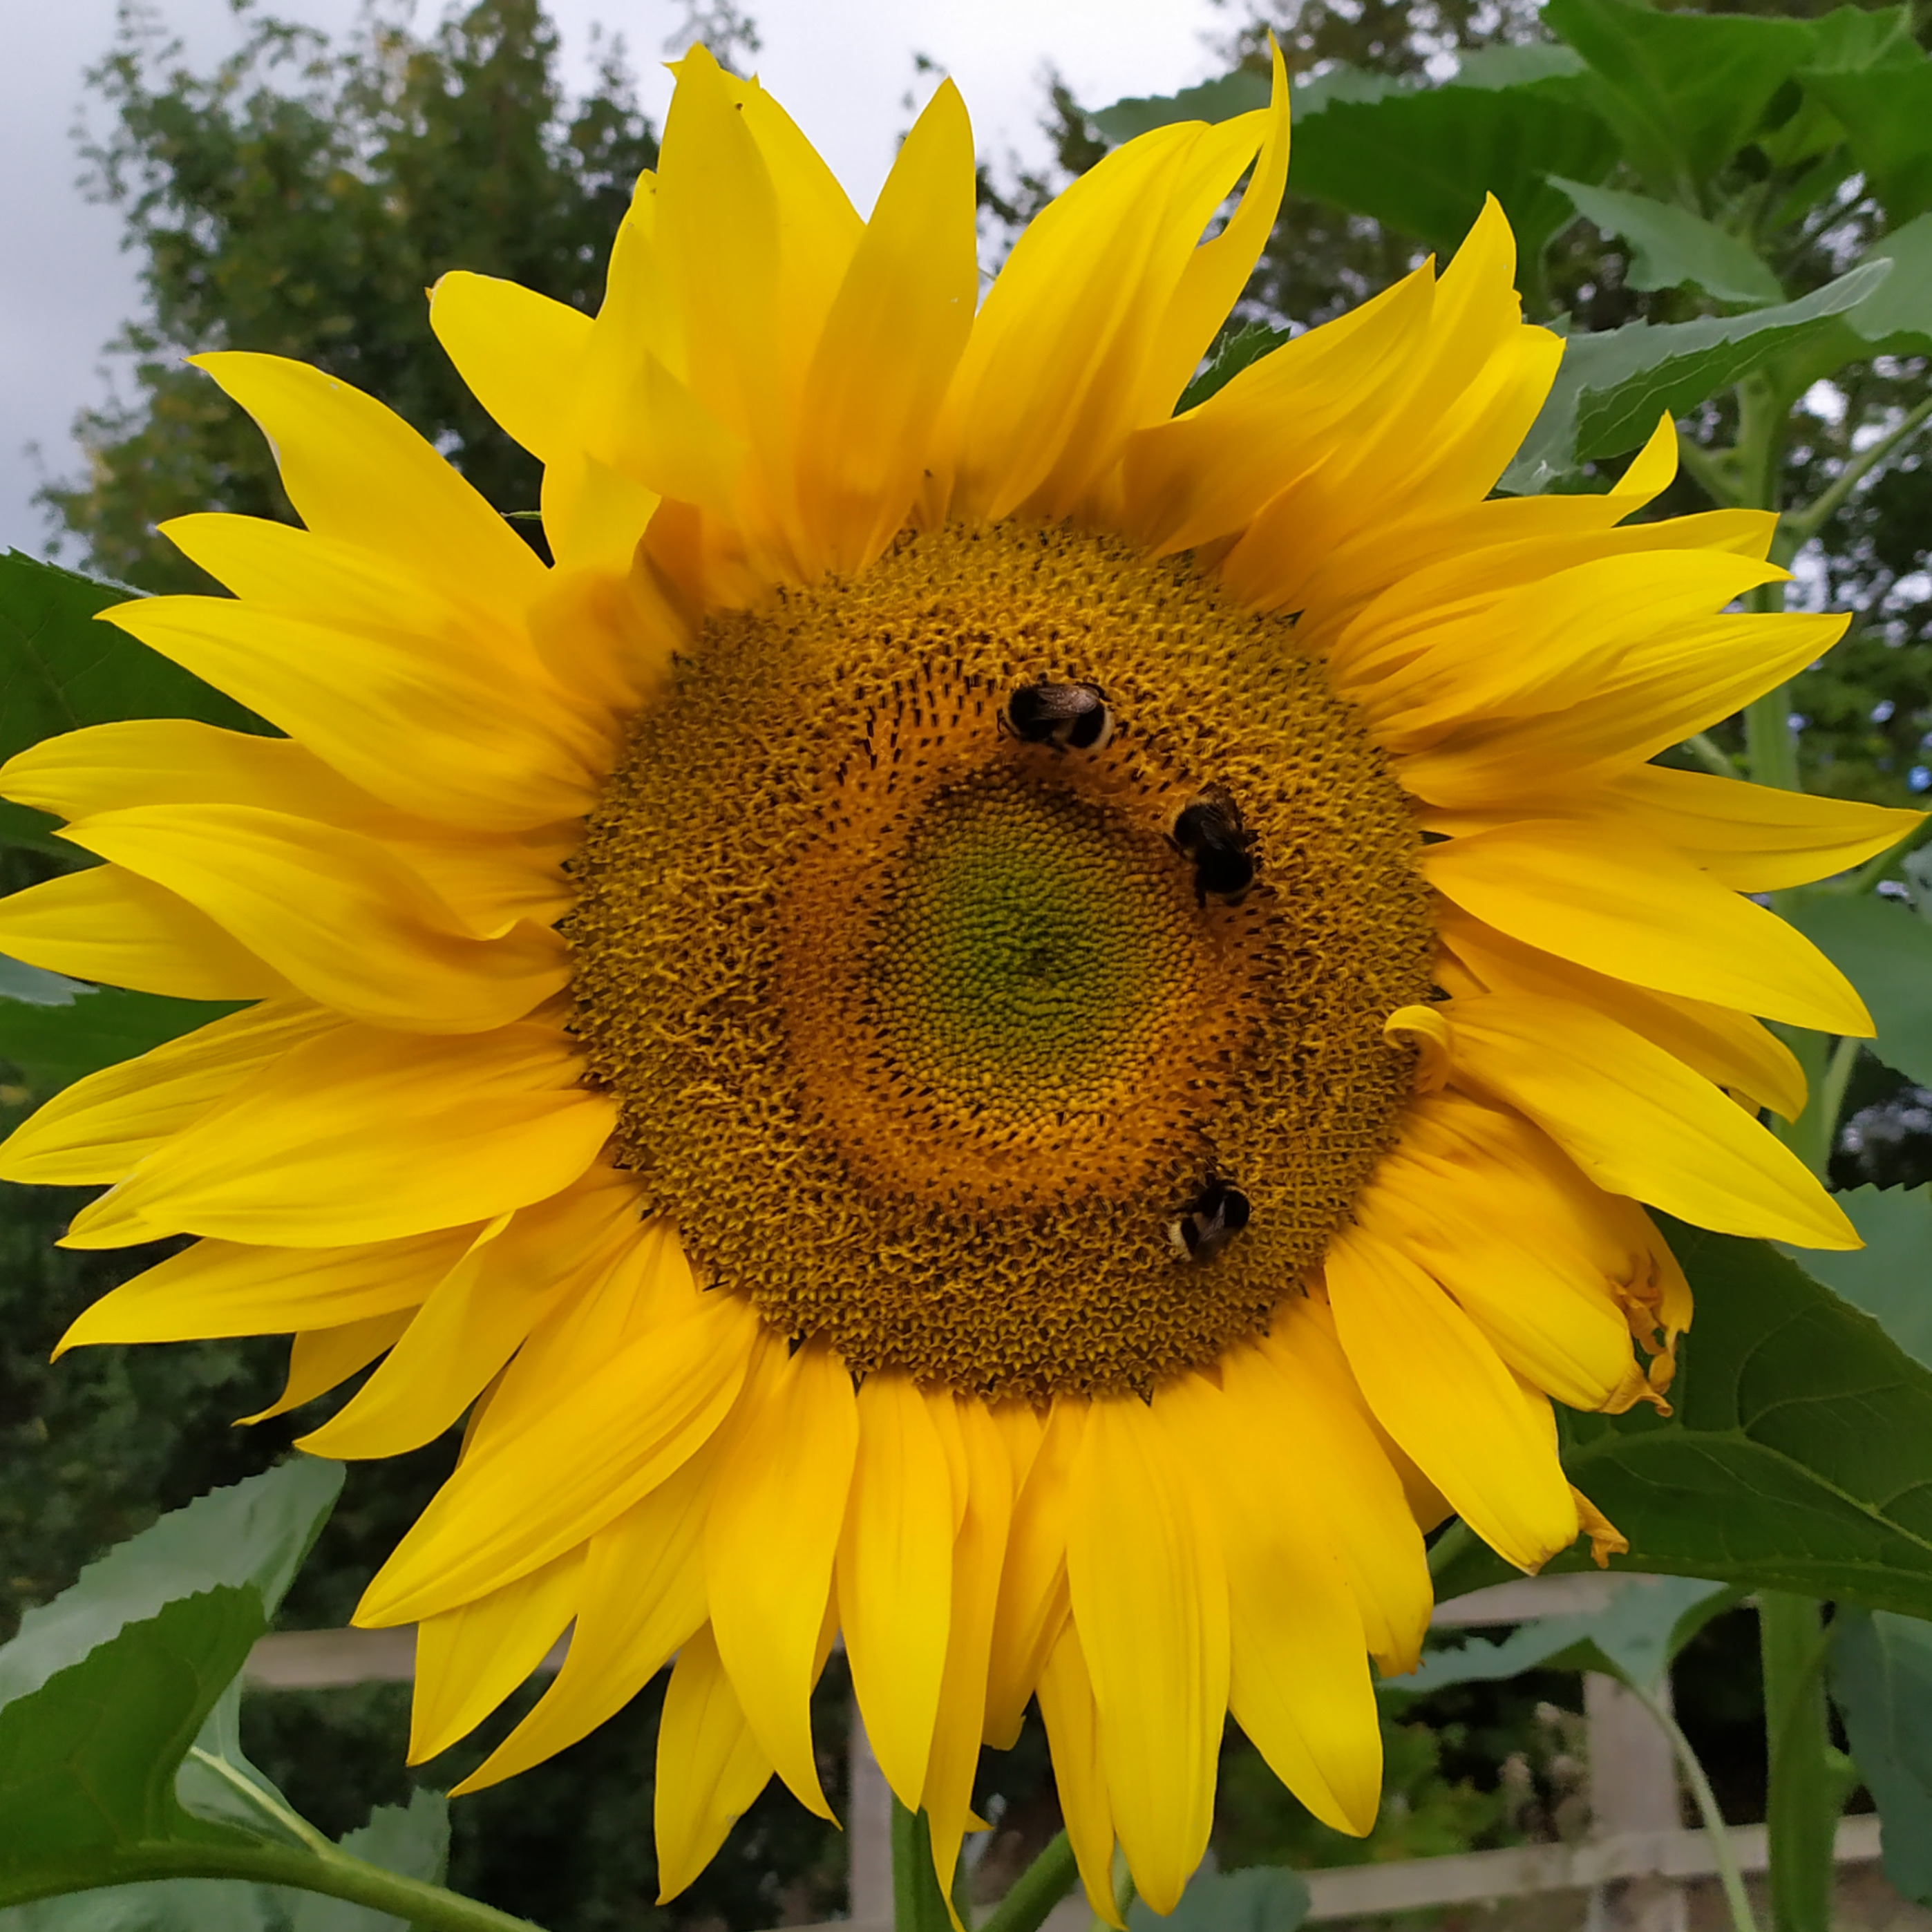
\includegraphics[height=0.7cm]{sunflower.jpg}}

% Frametitle template with line break and consistent image
\setbeamertemplate{frametitle}{%
  \begin{beamercolorbox}[wd=\paperwidth,ht=3ex,dp=1ex]{frametitle}
    \hspace*{1em}
    \usebeamerfont{frametitle}\insertframetitle\par
    \hfill
    \raisebox{-0.7ex}{\frametitleimage}
  \end{beamercolorbox}%
}

\transdissolve

% Bookmark for the title page (level 1)
\AtBeginDocument{
  \pdfbookmark[1]{Title Page}{titlepage}
}

% Section page bookmarks (level 1)
\AtBeginSection[]{
  \begin{frame}
    \transdissolve
    \pdfbookmark[1]{\insertsection}{section:\insertsection}
    \frametitle{\insertsection}
    \vspace{0.5cm}
  \end{frame}
}

% Frame bookmarks with slide numbers (level 1)
\setbeamertemplate{frametitle}{%
  \pdfbookmark[1]{\insertframenumber. \insertframetitle}{frame:\insertframenumber}
  \begin{beamercolorbox}[wd=\paperwidth,ht=3ex,dp=1ex]{frametitle}
    \hspace*{1em}
    \usebeamerfont{frametitle}\insertshortframetitle
    \hfill
    \raisebox{-0.7ex}{\frametitleimage} % Consistent image
  \end{beamercolorbox}%
}

% Command to define a shorter frametitle for bookmarks
\newcommand{\shortframetitle}[1]{
  \gdef\insertshortframetitle{#1}
}
